\documentclass{article}
\usepackage{graphicx} % Para incluir imágenes
\usepackage[spanish]{babel}
\usepackage{makeidx}
\usepackage{geometry}
\usepackage{amsmath}
\usepackage{graphicx}
\usepackage{caption}
\usepackage{pdfpages}
\usepackage{hyperref}
\usepackage{placeins}
\hypersetup{
    colorlinks,
    citecolor=black,
    filecolor=black,
    linkcolor=black,
    urlcolor=black
}



\geometry{a4paper, total={170mm,257mm}, left=20mm, top=20mm}
\renewcommand{\familydefault}{\sfdefault}


\begin{document}
\begin{titlepage}
    \centering
    \Large
    Universidad Central de Venezuela\\
    Facultad de Ingeniería\\
    Escuela de Ingeniería Eléctrica
    \vspace*{8cm}

    \Huge
    \textbf{Prelaboratorio Nº 4:} 

    \textbf{Respuesta en frecuencia}
    \vfill


    \Large

    Emerson Warhman \\
    C.I. 25.795.480 \\
    \today

\end{titlepage}
\tableofcontents
\newpage

\section{Introducción}

Los amplificadores operacionales (op-amps) son dispositivos versátiles que encuentran aplicaciones tanto en circuitos lineales como no lineales. Mientras que en configuraciones lineales se utilizan principalmente para operaciones de amplificación y filtrado, sus aplicaciones no lineales abren un panorama de posibilidades en generación y conformación de señales. Este informe explora tres configuraciones fundamentales de op-amps en régimen no lineal: el oscilador de puente de Wien, los multivibradores (astable y monoestable) y los generadores de funciones.

El \textbf{oscilador de puente de Wien} representa una aplicación clásica en generación de señales sinusoidales. Su diseño aprovecha el balance entre una red de realimentación positiva (para mantener las oscilaciones) y un mecanismo de control de amplitud (usualmente mediante diodos o JFETs) que garantiza estabilidad en la señal de salida. La frecuencia de oscilación está determinada por la relación $f_o = \frac{1}{2\pi RC}$, demostrando cómo componentes pasivos simples pueden definir características fundamentales de la señal generada.

Los \textbf{multivibradores} ilustran la capacidad de los op-amps para trabajar en conmutación:
\begin{itemize}
    \item El \textbf{astable} opera como oscilador libre, generando una onda cuadrada continua cuya frecuencia depende de los elementos RC en el circuito
    \item El \textbf{monoestable} produce un pulso de duración fija ante un disparo externo, siendo útil en aplicaciones de temporización
\end{itemize}

Los \textbf{generadores de funciones} amplían estas capacidades para producir formas de onda complejas (triangulares, diente de sierra, etc.), a menudo mediante la integración controlada de señales cuadradas. Estos circuitos encuentran aplicaciones prácticas en sistemas de comunicaciones, instrumentación médica y equipos de prueba electrónicos.

Este estudio experimental permitirá verificar los principios teóricos de operación, analizar las relaciones entre los componentes y los parámetros de salida, y evaluar las limitaciones prácticas de estos circuitos. Particular atención se dedicará al análisis de distorsión armónica en el oscilador Wien y a la precisión temporal en los multivibradores, aspectos críticos para aplicaciones reales.



\section{Resumen}

\subsection{Generador de funciones}

La onda exponencial generada en un circuito astable puede ser cambiada a un una onda triangular reemplazando el circuito RC con un integrador cómo se muestra en la ilustración . El integrador ocaciona que el capacitor se cargue y descargue de manera lineal, obteniendo de esta forma una onda triangular. \cite[pag. ~1366]{sedra-smith}

\begin{ilustracion}[ht]
    \centering
    \includegraphics[width=0.5\textwidth]{marco-teorico/generador-funciones.png}
    \caption{Generador de funciones}
\end{ilustracion}

Supongamos que en la salida $V_{SQ}$ del circuito tenemos valores máximos $V_{SQ+}$ y mínimos $V_{SQ-}$, Cuando el valor de la salida es $V_{SQ+}$ una corriente es $V_{SQ+}/R$ va a pasar a traves de la resistencia y del condensador, causando que en la salida del integrador decrezca linealmente con una pendiente $-V_{SQ+}/RC$, Esto va a ocurrir hasta que la salida del integrador alcance el límite inferior del circuito astable, punto en el cual es circuito astable cambiará de estado, volviendose la salida del astable igual a $V_{SQ-}$. En este momento la corriente a traves de R y C cambiará de dirección y su valor se volverá $-V_{SQ-}/R$, causando que la salida del integrador aumente linealmente con una pendiente $V_{SQ-}/RC$ hasta que alcance el límite superior del circuito astable, punto en el cual el circuito astable cambiará de estado, volviendose la salida del astable igual a $V_{SQ+}$, una vez alcanzado este punto el circuito cambiará de estado nuevamente, haciendo que el voltaje en su salida sea $V_{SQ+}$ y repitiendo el ciclo.

De lo dicho anteriormente se puede deducir una expresión para el periodo $T$ de la onda triangular y la onda cuadrada. Durante el intervalo $T_1$ tenemos

\begin{equation*}
    \frac{V_{TH} - V_{TL}}{T_1} = \frac{V_{SQ+}}{RC}
\end{equation*}

de donde podemos despejar $T_1$

\begin{equation}
    T_1 = \frac{V_{TH} - V_{TL}}{V_{SQ+}}RC
    \label{eq:t1}
\end{equation}

De manera similar, durante $T_2$ tenemos

\begin{equation*}
    \frac{V_{TH} - V_{TL}}{T_2} = \frac{-V_{SQ-}}{RC}
\end{equation*}

de donde podemos despejar $T_2$

\begin{equation}
    T_2 = \frac{V_{TH} - V_{TL}}{-V_{SQ-}}RC
\end{equation}

\section{Metodología}

Se estudiará el comportamiento de cada etapa por separado del circuito base, el circuito completo, la respuesta en frecuencia, al circuito realimentado.

\begin{figure}[ht]
    \centering
    \includegraphics[width=0.9\textwidth]{src/images/metodología/circuito-base.png}
    \caption{Circuito base}
    \label{fig:met-circuito-base}
\end{figure}
    
\subsection{Análisis de la etapa de potencia}


\begin{itemize}
    \item Al medir los puntos de operación en la etapa de potencia podemos observar que el máximo error en la medición de voltaje $V_{ce}$ es de tan solo $4.84\%$ por lo que nuestra predeterminación para este valor es correcto. Por otro lado podemos observar que el error en la medición $I_c$ está entre 60\% y 529\%, estos errores son grandísimos, esto se puede deber a que dichas corrientes de colector son muy pequeñas.
    \item Para el modelo dinámico del amplificador podemos observar que la impedancia de entrada $Z_i$ tiene un error de solo $7.15\%$ siendo un valor aceptable, igualmente la medición de ganancia tiene un error de $3.85\%$ indicando que la predeterminación es correcta, por su parte la medición de impedancia de salida $Z_o$ tiene un error de $91.16\%$ lo cual es muy alto. El valor de la medición es de 11, lo cual se acerca más al valor de la resistencia $r_{13} = 100\Omega$.
    \item Al modificar la etapa para que se comporte como un amplificador clase C podemos observar que los voltajes $V_{ce}$ medidos corresponden con los teóricos, mientras que las corrientes $I_e$ medidas siguen teniendo un error altísimos. No se observan cambios notables entre el punto de operación del amplificador clase C y el AB. 
    \item En la ilustración \ref{ilus:efecto-crossover-amplificador-clase-c} podemos observar el efecto crossover del amplificador clase C el cual consiste en una pequeña distorsión en la zona de cruce de la onde. No se persive ningún cambio en la ganancia con respecto al otro modo. .
\end{itemize}

\section{Resultados}

\section{Análisis de resultados}

\section{Conclusiones}

\section{Anexos}
\section{Anexos}

\begin{ilustracion}[ht]
    \centering
    \includegraphics[width=1.0\textwidth]{src/images/p1/p1-hoja-de-datos.jpg}
    \caption{Hoja de datos práctica N° 1}
    \label{ilus:hoja-de-datos-p1}
\end{ilustracion}

\begin{ilustracion}[ht]
    \centering
    \includegraphics[width=1.0\textwidth]{src/images/p2/p2-hoja-de-datos.jpg}
    \caption{Hoja de datos práctica N° 2}
    \label{ilus:hoja-de-datos-p2}
\end{ilustracion}

\begin{ilustracion}[ht]
    \centering
    \includegraphics[width=1.0\textwidth]{src/images/p3/p3-hoja-de-datos.jpg}
    \caption{Hoja de datos práctica N° 3-1}
    \label{ilus:hoja-de-datos-p3-1}
\end{ilustracion}

\begin{ilustracion}[ht]
    \centering
    \includegraphics[width=1.0\textwidth]{src/images/p3/p3-hoja-de-datos-2.jpg}
    \caption{Hoja de datos práctica N° 3-2}
    \label{ilus:hoja-de-datos-p3-2}
\end{ilustracion}

\begin{ilustracion}[ht]
    \centering
    \includegraphics[width=1.0\textwidth]{src/images/p4/p4-hoja-de-datos-1.jpg}
    \caption{Hoja de datos práctica N° 4-1}
    \label{ilus:hoja-de-datos-p4-1}
\end{ilustracion}

\begin{ilustracion}[ht]
    \centering
    \includegraphics[width=1.0\textwidth]{src/images/p4/p4-hoja-de-datos-2.jpg}
    \caption{Hoja de datos práctica N° 4-2}
    \label{ilus:hoja-de-datos-p4-2}
\end{ilustracion}

\begin{ilustracion}[ht]
    \centering
    \includegraphics[width=1.0\textwidth, angle=90]{src/images/p5/p5-hoja-de-datos-1.jpg}
    \caption{Hoja de datos práctica N° 5-1}
    \label{ilus:hoja-de-datos-p5-1}
\end{ilustracion}

\begin{ilustracion}[ht]
    \centering
    \includegraphics[width=1.0\textwidth,angle=90]{src/images/p5/p5-hoja-de-datos-2.jpg}
    \caption{Hoja de datos práctica N° 5-2}
    \label{ilus:hoja-de-datos-p5-2}
\end{ilustracion}

\begin{ilustracion}[ht]
    \centering
    \includegraphics[width=1.0\textwidth, angle=90]{src/images/p5/p5-hoja-de-datos-3.jpg}
    \caption{Hoja de datos práctica N° 5-3}
    \label{ilus:hoja-de-datos-p5-3}
\end{ilustracion}

\includepdf[page=-, width=0.9\textwidth]{src/assets/BC237.pdf}
\captionof{ilustracion}{Hoja de datos del transistor BC237}

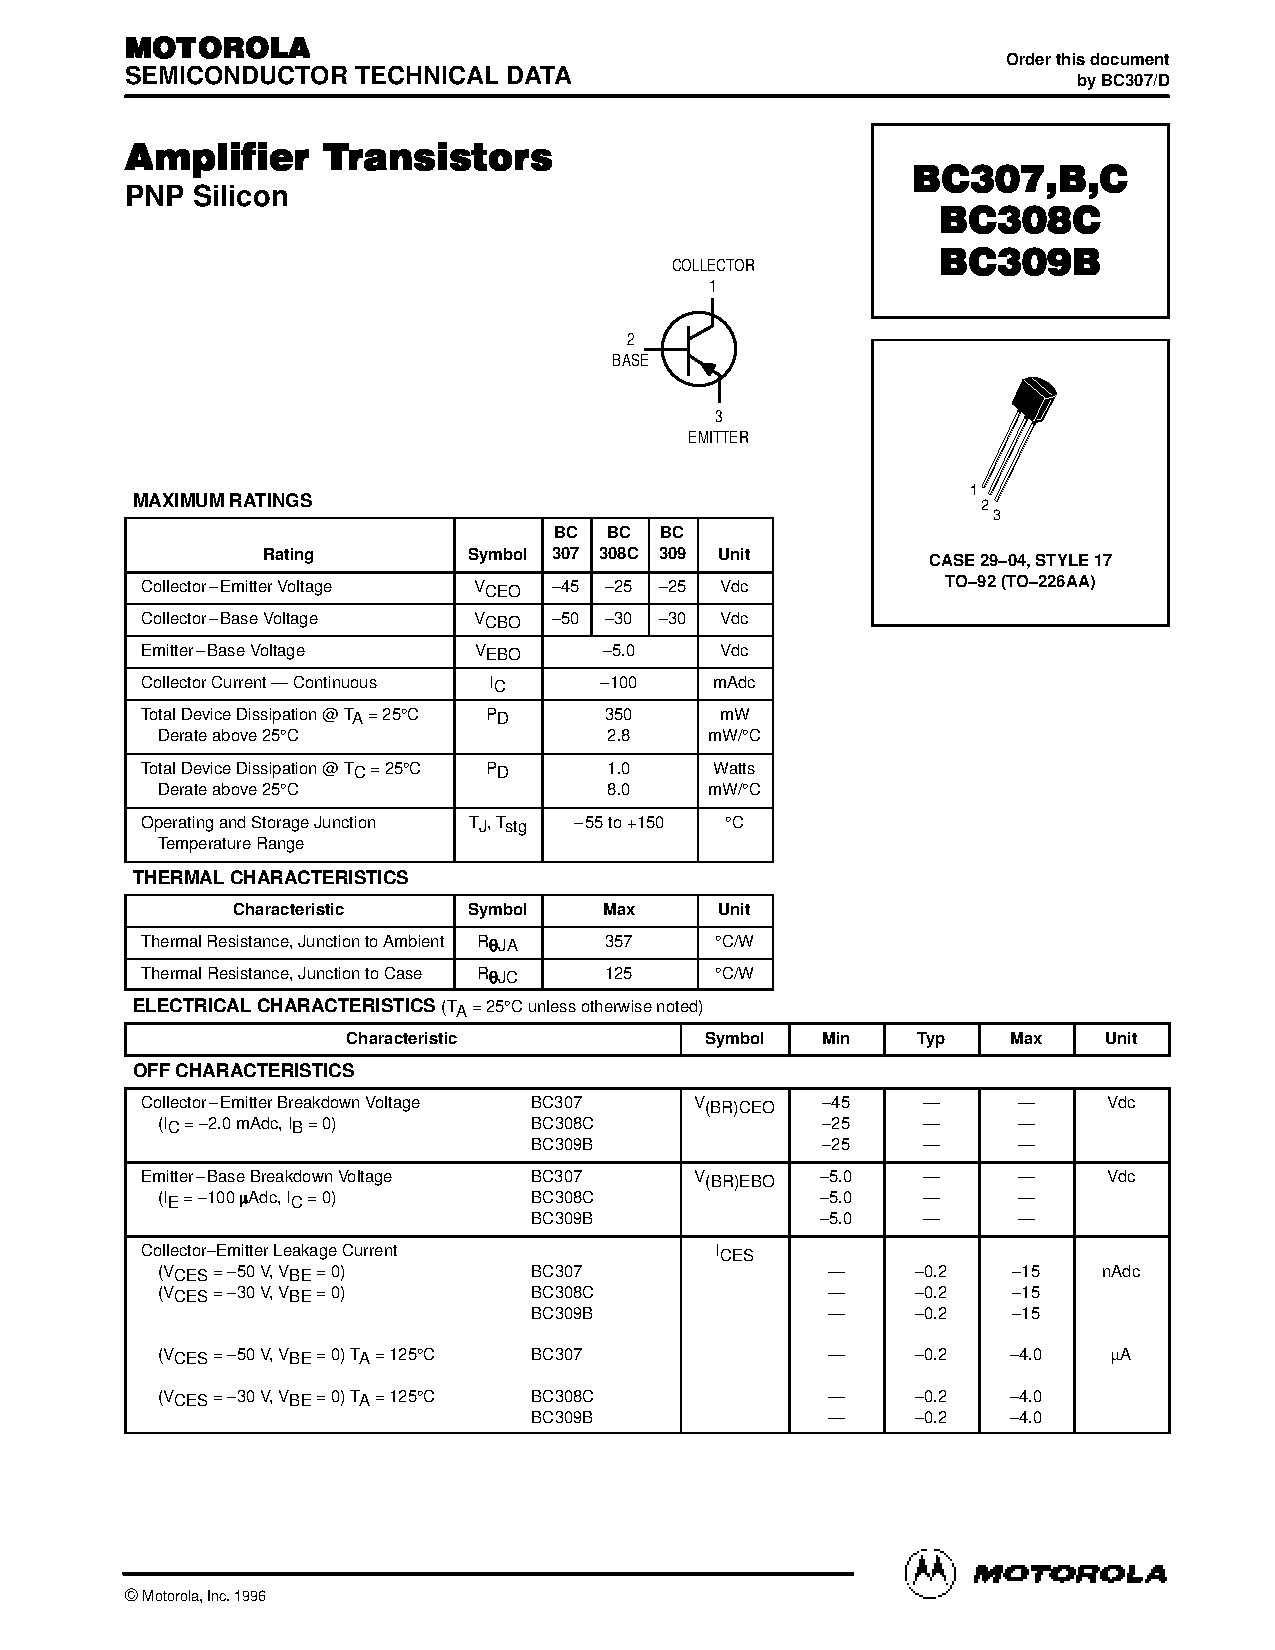
\includepdf[page=-, width=0.9\textwidth]{src/assets/bc307.pdf}
\captionof{ilustracion}{Hoja de datos del transistor BC307}


\end{document}
